\PassOptionsToPackage{usenames}{xcolor}
\PassOptionsToPackage{dvipsnames}{xcolor}
\documentclass[11pt,a4paper,twoside,final,titlepage,openright,fleqn]{book}%
\usepackage{beamerarticle}

\usepackage[utf8]{inputenc}
\usepackage[T1]{fontenc}
\usepackage[spanish]{babel}

\usepackage{listings}
\usepackage{palatino}
\usepackage{lmodern}

%\renewcommand*\rmdefault{lmr}
%\renewcommand*\ttdefault{ppl}

\usepackage{url}
\usepackage{multicol}

\usepackage{tabularx}

\usepackage{tikz}
\usetikzlibrary{positioning}
\usetikzlibrary{arrows}
\usetikzlibrary{mindmap}

\usepackage{pgfplots}
\pgfplotsset{compat=1.5}

\usepackage{ccicons}

\tikzset{
  invisible/.style={opacity=0},
  visible on/.style={alt=#1{}{invisible}},
  alt/.code args={<#1>#2#3}{%
    \alt<#1>{\pgfkeysalso{#2}}{\pgfkeysalso{#3}} % \pgfkeysalso doesn't change the path
  },
  bloque/.style={rectangle,draw=black, top color=white, bottom color=blue!50,
                 very thick, inner sep=0.5em, minimum size=0.6cm, text centered, font=\tiny},
  bloquelibre/.style={rectangle,draw=black, top color=white, bottom color=blue!10,
                 very thick, inner sep=0.5em, minimum size=0.6cm, text centered, font=\tiny},
  flecha/.style={->, >=latex', shorten >=1pt, thick},
  etiqueta/.style={text centered, font=\tiny} 
}



\usepackage[a4paper,left=2cm,right=2cm,top=2.5cm,bottom=4cm]{geometry}
\usepackage[colorlinks=true,linkcolor=blue,citecolor=blue,urlcolor=blue,plainpages=false,bookmarksnumbered=true,pdfpagemode=UseOutlines]{hyperref}


\usepackage[nottoc]{tocbibind}

%\usepackage[fixlanguage]{babelbib}


\usepackage{graphicx}
\usepackage{xcolor}
\usepackage{tikz}
\usetikzlibrary{arrows,positioning} 

\newcommand{\textgood}[1]{%
{\color{blue!60!black}\textbf{#1}}%
}

\newcommand{\textbad}[1]{%
{\color{red!80!black}\textbf{#1}}%
}

\newcommand{\textmark}[1]{%
{\color{orange!70!black}\textbf{#1}}%
}

\newcommand{\textenum}[1]{%
{\color{blue!60!black}\textbf{#1}}%
}

\newcommand{\textemph}[1]{%
{\color{green!40!black}\textbf{#1}}%
}

\newcommand{\versionid}{2021.1}
\newcommand{\versiondate}{Noviembre de 2021}

\newcommand{\coursetitle}{Programación paralela en C++ moderno}
\newcommand{\moduleintro}{Introducción a la programación paralela}
\newcommand{\modulepatrones}{Patrones de paralelismo en oneTBB}


\newtheorem{ejer}{Ejercicio}

\usepackage{url}

\usepackage{pdfpages}

\usepackage{todonotes}

%Package fancyhdr
\usepackage{fancyhdr}
\setlength{\headheight}{1.7cm}%{13.6pt}
\pagestyle{fancyplain}
\fancyhf{}
\lhead{
\includegraphics[height=1.25cm]{logos/uc3m.png}}
\chead{}
\rhead{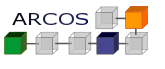
\includegraphics[height=1.25cm]{logos/arcos.png}}
\rfoot{\begin{tabular}{r}\coursetitle\\Versión \versionid\end{tabular}}
\cfoot{\begin{tabular}{c}{\thepage}\\{}\end{tabular}}
\lfoot{
\begin{tabular}{l}
\textbf{\ccbysa} -- CC BY-SA 4.0\\J. Daniel Garcia -- ARCOS@UC3M
\end{tabular}
}
\renewcommand{\headrulewidth}{0.5pt} % remove lines as well
\renewcommand{\footrulewidth}{0.5pt}
\renewcommand{\plainheadrulewidth}{0.5pt}
\renewcommand{\plainfootrulewidth}{0.5pt}

\renewcommand{\topfraction}{0.9}
\renewcommand{\textfraction}{0.1}
\renewcommand{\floatpagefraction}{0.9}

\usepackage{palatino}
\usepackage{lmodern}

\renewcommand*\rmdefault{lmr}
\renewcommand*\ttdefault{ppl}

\makeindex

\begin{document}

\mode<article>{
\lstset{
  language=C++,
  belowcaptionskip=1\baselineskip,
  breaklines=true,
  xleftmargin=\parindent,
  showstringspaces=false,
  basicstyle=\small,
  keywordstyle=\bfseries\color{green!40!black},
  commentstyle=\itshape\color{purple!40!black},
  identifierstyle=\color{blue},
  stringstyle=\color{brown},
  columns=fullflexible,
  inputencoding=utf8,
  extendedchars=true,
  upquote=true,
  morekeywords=[1]{_Pragma,constexpr,nullptr,alignof,alignas,decltype,override,final,noexcept,deprecated,thread_local,co_await,co_return,co_yield,fallthrough},
  literate=%
    {¿}{{?`}}{1}
    {¡}{{!`}}{1}
    {á}{{\'a}}{1}
    {é}{{\'e}}{1}
    {í}{{\'i}}{1}
    {ó}{{\'o}}{1}
    {ú}{{\'u}}{1}
    {ñ}{{\~n}}{1}
}
}

\mode<presentation>{
\lstset{
  language=C++,
  belowcaptionskip=1\baselineskip,
  breaklines=true,
  xleftmargin=\parindent,
  showstringspaces=false,
  basicstyle=\scriptsize,
  keywordstyle=\bfseries\color{green!40!black},
  commentstyle=\itshape\color{purple!40!black},
  identifierstyle=\color{blue},
  stringstyle=\color{orange},
  directivestyle=\bfseries\color{green!40!black},
  columns=fullflexible,
  inputencoding=utf8,
  extendedchars=true,
  upquote=true,
  morekeywords=[1]{_Pragma,constexpr,nullptr,alignof,alignas,decltype,override,final,noexcept,deprecated,thread_local,co_await,co_return,co_yield,fallthrough},
  literate=%
    {¿}{{?`}}{1}
    {¡}{{!`}}{1}
    {á}{{\'a}}{1}
    {é}{{\'e}}{1}
    {í}{{\'i}}{1}
    {ó}{{\'o}}{1}
    {ú}{{\'u}}{1}
    {ñ}{{\~n}}{1}
}
}

\newcommand{\cppkey}[1]{%
{\color{green!40!black}\textbf{#1}}%
}

\newcommand{\cppid}[1]{%
{\color{blue}\textbf{#1}}%
}

\newcommand{\cppstr}[1]{%
{\color{orange}\textbf{#1}}%
}


\lstdefinestyle{terminal}{
  language=bash,
  basicstyle=\scriptsize\ttfamily,
  numbersep=3pt,
  frame=tb,
  columns=fullflexible,
  backgroundcolor=\color{yellow!20},
}



\frontmatter

\pagestyle{empty}
\begin{titlepage}
\tikz[remember picture,overlay] \draw [fill,Blue] (current page.north west) rectangle +(0.2\paperwidth,-\paperheight);
\begin{flushright}

\includegraphics[width=5cm]{logos/uc3m.png}
\\
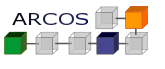
\includegraphics[width=5cm]{logos/arcos.png}
\end{flushright}

\vfill

\begin{tabular}{p{3cm}l}
&
\LARGE{Material de curso}
\\

&\\

&
\LARGE{\coursetitle}
\\

&\\

&
Version: \versionid
\\

&
\versiondate
\\

\end{tabular}
\vfill
\begin{tabular}{p{3cm}l}
&José Daniel García Sánchez\\
&Departamento de Informática\\
&Universidad Carlos III de Madrid\\
&Av. Universidad, 30\\
&28911 Leganés, Madrid\\
&\url{josedaniel.garcia@uc3m.es}\\
\end{tabular}
\vspace{1cm}
\\
\begin{tabular}{p{3cm}l}
&
%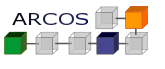
\includegraphics[width=5cm]{logos/arcos.png}
%\includegraphics[width=8cm]{logos/logo-uc3m.jpg}
\\
\end{tabular}
\end{titlepage}

\pagestyle{fancyplain}
\chapter*{Atribución-CompartirIgual 4.0 Internacional (CC BY-SA 4.0)}

Este es un resumen legible por humanos (y no un sustituto) de la
(código legal disponible en
\url{https://creativecommons.org/licenses/by-sa/4.0/legalcode}
).

\section*{Usted es libre de:}

\begin{itemize}

\item \textbf{Compartir} --
copiar y redistribuir el material en cualquier medio o formato.

\item \textbf{Adaptar} -- 
remezclar, transformar y construir a partir del material
para cualquier propósito, incluso comercialmente.

\end{itemize}

La licenciante no puede revocar estas libertades en tanto usted siga los
términos de la licencia.

\section*{Bajo los siguientes términos:}

\begin{itemize}

\item \ccAttribution \quad \textbf{Atribución} --
Usted debe dar crédito de manera adecuada, brindar un enlace a la licencia, e
indicar si se han realizado cambios. Puede hacerlo en cualquier forma
razonable, pero no de forma tal que sugiera que usted o su uso tienen el apoyo
de la licenciante. 

\item \ccShareAlike \quad \textbf{CompartirIgual} --
Si remezcla, transforma o crea a partir del material, debe distribuir su
contribución bajo la lamisma licencia del original. 

\item \textbf{No hay restricciones adicionales} -- 
No puede aplicar términos legales ni medidas tecnológicas que restrinjan
legalmente a otras a hacer cualquier uso permitido por la licencia. 

\end{itemize}

\section*{Avisos:}

No tiene que cumplir con la licencia para elementos del materiale en el dominio
público o cuando su uso esté permitido por una excepción o limitación
aplicable.

No se dan garantías. La licencia podría no darle todos los permisos que
necesita para el uso que tenga previsto. Por ejemplo, otros derechos como
publicidad, privacidad, o derechos morales pueden limitar la forma en que
utilice el material.


\cleardoublepage
\chapter*{Presentación}

Bienvenidos al curso de programación paralela en C++ moderno.


\section*{Structure}

Los contenidos de este curso se estructuran de la siguiente forma:

\begin{enumerate}

\item \ldots

\end{enumerate}

\cleardoublepage
\chapter*{Agradecimientos}

En primer lugar, me gustaría dar las gracias a mi amigo
Rafael Asenjo que me introdujo en el uso de TBB.

Así mismo, me gustaría agradecer de forma especial a todos aquellos
que han proporcionado realimentación sobre versiones previas de este 
material.


\cleardoublepage
\tableofcontents
\todototoc
\listoftodos

\mainmatter

\pagestyle{fancyplain}
\mode<article>{\chapter{\moduleintro}}

\mode<presentation>{\begin{frame}[shrink=20]{Licencia Creative Commons}

\begin{tabularx}{.98\textwidth}{lX}
\ccLogo & Este trabajo se distribuye bajo licencia
Atribución-NoComercial-SinDerivadas 4.0 Internacional (CC BY-NC-ND 4.0).\\

&\\

& \multicolumn{1}{c}{\textbf{Usted es libre de}:}\\

&\\

&
\textbf{Compartir} --
copiar y redistribuir el material en cualquier medio o formato.
\\

&\\

& \multicolumn{1}{c}{\textbf{Bajo los siguientes términos}:}\\

&\\

\ccAttribution &
Atribución -- Usted debe dar crédito de manera adecuada, brindar un enlace a la licencia, e indicar si se han realizado cambios. Puede hacerlo en cualquier forma razonable, pero no de forma tal que sugiera que usted o su uso tienen el apoyo de la licenciante.
\\

\ccNonCommercialEU &
NoComercial -- Usted no puede hacer uso del material con propósitos comerciales. 
\\

\ccNoDerivatives &
SinDerivadas -- Si remezcla, transforma o crea a partir del material, no podrá distribuir el material modificado. 
\\

\end{tabularx}

\end{frame}
}
\section{Visión general}

\begin{frame}[t]{¿Qué es oneTBB?}
\begin{itemize}
  \item \textgood{oneTBB}: One Threading Building Blocks.
    \begin{itemize}
      \item Evolución de Intel Threading Building Blocks.
    \end{itemize}

  \mode<presentation>{\vfill\pause}
  \item Una bibliteca para expresar el paralelismo.

  \mode<presentation>{\vfill\pause}
  \item \textemph{Características}:
    \begin{itemize}
      \item Permite especificar el \textmark{paralelismo lógico} en
            vez de \textbad{trabajar directamente con hilos}.
      \item Se centra el uso de hilos para \textgood{mejorar el rendimiento}.
      \item Pone el foco en la escalabilidad en el \textmark{paralelismo de datos}.
      \item Se apoya fuertemente en la \textmark{programación genérica}.
    \end{itemize}
\end{itemize}
\end{frame}

\begin{frame}[t]{Estructura de oneTBB}
\begin{itemize}

  \item \textmark{Algoritmos y estructuras paralelas}:
    \begin{itemize}
      \item Algoritmos genéricos paralelos.
      \item Grafos de flujo.
      \item Contenedores concurrentes.
    \end{itemize}

  \mode<presentation>{\vfill\pause}
  \item \textmark{Hilos y sincronización}:
    \begin{itemize}
      \item Primitivas de sincronización.
      \item Temporizadores y excepciones.
      \item Hilos.
      \item Almacenamiento local al hilo.
    \end{itemize}

  \mode<presentation>{\vfill\pause}
  \item \textmark{Memoria y planificación}:
    \begin{itemize}
      \item Planifcadores de tareas.
      \item Gestión de memoria.
    \end{itemize}
\end{itemize}
\end{frame}



\section{Procesando datos en paralelo}

\begin{frame}[t,fragile]{Procesando datos en un vector}
\begin{block}{Elevar al cuadrado}
\begin{lstlisting}
void square_seq(std::vector<int> &v) {
  for (auto &x : v) {
    x *= x;
  }
}
\end{lstlisting}
\end{block}

\mode<presentation>{\vfill\pause}
\begin{block}{Calcular el promedio}
\begin{lstlisting}
double average_seq(const std::vector<int> &v) {
  double s = 0.0;
  for (auto x : v) {
    s += x;
  }
  return s / static_cast<double>(v.size());
}
\end{lstlisting}
\end{block}
\end{frame}

\begin{frame}[t,fragile]{Proyecciones}
\begin{itemize}
  \item Se puede expresar la función cuadrado como una \textmark{proyección}
        con el algoritmo \cppid{std::transform()}
\end{itemize}

\mode<presentation>{\vfill\pause}
\begin{block}{Usando std::transform()}
\begin{lstlisting}
#include <algorithm>

void square_stl(std::vector<int> &v) {
  std::transform(v.begin(), v.end(), v.begin(),
                 [](auto x) { return x * x; });
}
\end{lstlisting}
\end{block}
\end{frame}

\begin{frame}[t,fragile]{Reducciones}
\begin{itemize}
  \item Se puede expresar la suma como una \textmark{reducción}
        con \cppid{std::reduce()}.
\end{itemize}

\mode<presentation>{\vfill\pause}
\begin{block}{Usando std::reduce()}
\begin{lstlisting}
#include <numeric>

double average_stl(const std::vector<int> &v) {
  double s = std::reduce(v.begin(), v.end(), 0.0,
                         [](auto x, auto y) { return x + y; });
  return s / static_cast<double>(v.size());
}
\end{lstlisting}
\end{block}
\end{frame}

\begin{frame}[t,fragile]{Versiones paralelas de la STL}
\begin{itemize}
  \item La mayoría de los algoritmos de la STL admiten un parámetro para indicar
        la política de ejecución:
    \begin{itemize}
      \item \cppid{std::execution:seq}:
            Ejecución secuencial.
      \item \cppid{std::execution:par}:
            Ejecución paralela.
      \item \cppid{std::execution:par\_unseq}:
            Ejecución paralela, vectorizada y/o migración entre hilos.
      \item \cppid{std::execution:unseq}:
            Ejecución vectorizada.
    \end{itemize}

\end{itemize}
\end{frame}

\begin{frame}[t,fragile]{Transformación}
\begin{block}{Transformación}
\begin{lstlisting}
void square_stlpar(std::vector<int> &v) {
  std::transform(std::execution::par,
      v.begin(), v.end(), v.begin(),
                 [](auto x) { return x * x; });
}

void square_stlunseq(std::vector<int> &v) {
  std::transform(std::execution::unseq,
                 v.begin(), v.end(), v.begin(),
                 [](auto x) { return x * x; });
}

void square_stlparunseq(std::vector<int> &v) {
  std::transform(std::execution::par_unseq,
                 v.begin(), v.end(), v.begin(),
                 [](auto x) { return x * x; });
}
\end{lstlisting}
\end{block}
\end{frame}

\begin{frame}[t,fragile]{Reducción}
\begin{block}{Reducción}
\begin{lstlisting}
double average_stlpar(const std::vector<int> &v) {
  double s = std::reduce(std::execution::par, v.begin(), v.end(), 0.0,
                         [](auto x, auto y) { return x + y; });
  return s / static_cast<double>(v.size());
}

double average_stlunseq(const std::vector<int> &v) {
  double s = std::reduce(std::execution::unseq, v.begin(), v.end(), 0.0,
                         [](auto x, auto y) { return x + y; });
  return s / static_cast<double>(v.size());
}

double average_stlparunseq(const std::vector<int> &v) {
  double s = std::reduce(std::execution::par_unseq, v.begin(), v.end(), 0.0,
                         [](auto x, auto y) { return x + y; });
  return s / static_cast<double>(v.size());
}
\end{lstlisting}
\end{block}
\end{frame}

\begin{frame}[t,fragile]{Paralelización con oneTBB}
\begin{itemize}
  \item Espacio de nombres \cppid{oneapi::tbb}.
\begin{lstlisting}
using namespace oneapi::tbb;
\end{lstlisting}

  \item Rango de iteración:
    \begin{itemize}
      \item Varios tipos de rangos en la biblioteca.
      \item Rango dentro de un bloque: \cppid{blocked\_range<T>}.
        \begin{itemize}
          \item \cppid{T} puede ser un tipo númerico o iterador.
        \end{itemize}
      \item Al paralelizar se opera sobre rangos.
    \end{itemize}
\end{itemize}
\end{frame}

\begin{frame}[t,fragile]{Cuadrado paralelo}
\begin{block}{parallel\_for()}
\begin{lstlisting}
void square_tbb(std::vector<int> &v) {
  using namespace oneapi::tbb;
  using range = blocked_range<std::vector<int>::iterator>;
  parallel_for(range{v.begin(), v.end()},
               [](const range &r) {
                 for (auto & x : r) {
                   x *= x;
                 }
               });
}
\end{lstlisting}
\end{block}
\end{frame}

\begin{frame}[t,fragile]{Suma paralela}
\begin{block}{parallel\_reduce()}
\begin{lstlisting}
double average_tbb(const std::vector<int> &v) {
  using namespace oneapi::tbb;
  using range_type = blocked_range<std::vector<int>::const_iterator>;
  double sum = parallel_reduce(
      range_type{v.begin(), v.end()}, 0.0,
      [](const range_type &r, double x) -> double {
        for (double value : r) {
          x += value;
        }
        return x;
      },
      [](auto x, auto y) { return x + y; });
  return sum / static_cast<double>(v.size());
}
\end{lstlisting}
\end{block}
\end{frame}

\begin{frame}[t,fragile]{Cuadrado paralelo + STL}
\begin{block}{parallel\_for()}
\begin{lstlisting}
void square_tbb(std::vector<int> &v) {
  using namespace oneapi::tbb;
  using range = blocked_range<std::vector<int>::iterator>;
  parallel_for(range{v.begin(), v.end()},
               [](const range &r) {
                 std::transform(r.begin(), r.end(), r.begin(),
                                [](auto x) { return x * x; });
               });
}
\end{lstlisting}
\end{block}
\end{frame}

\begin{frame}[t,fragile]{Suma paralela}
\begin{block}{parallel\_reduce()}
\begin{lstlisting}
double average_tbb(const std::vector<int> &v) {
  using namespace oneapi::tbb;
  using range_type = blocked_range<std::vector<int>::const_iterator>;
  double sum = parallel_reduce(
      range_type{v.begin(), v.end()}, 0.0,
      [](const range_type &r, double x) -> double {
        return std::reduce(r.begin(), r.end(), x);
      },
      [](auto x, auto y) { return x + y; });
  return sum / static_cast<double>(v.size());
}
\end{lstlisting}
\end{block}
\end{frame}




\nocite{*}
\bibliographystyle{abbrv}
\bibliography{bib/cppref}

\end{document}
